\documentclass[10pt]{article}
\usepackage{sdss2020} % Uses Times Roman font (either newtx or times package)
\usepackage{url}
\usepackage{latexsym}
\usepackage{amsmath, amsthm, amsfonts}
\usepackage{algorithm, algorithmic}  
\usepackage{multirow,graphicx}
\usepackage[flushleft]{threeparttable}
\usepackage[T1]{fontenc}
\usepackage{booktabs}
\usepackage{siunitx} 
\graphicspath{ {./images/} }

\newcolumntype{L}[1]{>{\raggedright\let\newline\\\arraybackslash\hspace{0pt}}m{#1}}
\newcolumntype{C}[1]{>{\centering\let\newline\\\arraybackslash\hspace{0pt}}m{#1}}
\newcolumntype{R}[1]{>{\raggedleft\let\newline\\\arraybackslash\hspace{0pt}}m{#1}}

\title{Modeling Opening Weekend Box Office Revenue for U.S. Movies, 2005-2007}

\author{
  C. Logue \\
  Georgetown University \\
  Washington, DC \\
\\\And
  P. Mernagh \\
  Georgetown University \\
  Washington, DC \\
\\\And
  Z. Holden \\
  Georgetown University \\
  Washington, DC \\
\\}

\begin{document}
\maketitle

\section{Introduction}
The project objective is to predict as accurately as possible opening weekend box office revenue for a set of movies, specifically from 2005-2007. Motivation for this project is a wealth of data points from both The Movie Database (TMDB) and Internet Movie Database (IMDb) around historical movies and TV shows: user-submitted ratings, applicable genres, budget, release date, actors, producer(s), production companies, country (or countries) of origin, etc. Further motivation is a prior understanding of likely useful predictors, such as the movie's budget, or the seasonal factors affecting a movie release. For example, the periods January-February, and to a lesser extent August-September, have been referred to as the ``dump months, '' i.e. effectively a dumping ground for low-potential movies that are not expected to make as much money. Various factors such as the seasonality of consumer spending (i.e binge before the holidays, pay down debt later), the timing of Golden Globes and Oscars awards, weather, the Super Bowl, and vacation months may all lead to seasonality in box office receipts.  The years 2005-2007 are specifically chosen since they predate the rise of the streaming era and its potential impacts on box office sales. They are a short enough period that no inflation adjustment is made to any financial variables. 
\section{Data}

Data on approximately 500 movies that opened in U.S. theaters between 2005-2007 was aggregated from TMDB and IMDb. Only English-language movies are included. Retrieved data points include the release date, the opening weekend revenue, budget, and the number of theaters the movie opened in. A selection of genres that each movie could be classified as (e.g. drama, thriller, action, crime, documentary, etc.) is included. Most movies are tagged with two to three genres, though a handful go as high as six. Popularity, a proprietary TMDB metric, is also included. It itself is based on various data points including votes, views, release date, etc.. As a community-built database, TMDB provides the data point vote average, namely the mean of user-submitted ratings on the scale of 0-10, as well as the number of submitted votes.  Both the origin and production country (or countries) are included. The production companies are provided (e.g big hitters such as Paramount, Warner Bros, MGM). Finally, the runtime, and what collection the movie belongs to, if any, such as the Harry Potter series or the Pirates of the Caribbean collection. The operating revenue and number of opening theaters were specifically pulled from Box Office Mojo, a service of IMDB Pro. The following predictors are chosen for initial modeling:
\begin{enumerate}
\item Budget (continuous)
\item Runtime (continuous)
\item Number of production companies (continuous)
\item From a series (binary, 118 total)
\item Opening weekend season (categorical)
\begin{enumerate}
\item Winter: January-February (71 total)
\item Spring: March-April (84 total)
\item Summer: May-August (154 total)
\item Fall: September-October (120 total)
\item Holiday: November-December (82 total)
\end{enumerate}
\end{enumerate}

Summary statistics are as follows:
\begin{table}[H]
\centering
\caption{Summary Statistics (n = 511)}
\begin{tabular}{lrrr} 
\toprule
Variable & Mean & Min & Max \\ 
\midrule
opening revenue (\$) & 14,743,982 & 9,653 & 151,116,516\\
budget (\$) & 40,365,469 & 0 & 300,000,000\\
runtime (min) & 107 & 14 & 187\\
\# of prod. cos. & 3.8 & 0 & 17\\
\bottomrule
\end{tabular}  
\end{table}

The variable popularity is not considered, since it is modeled by TMDB and likely influenced by post-opening weekend factors. The number of theaters the movie opened in is likely highly correlated with opening revenue. However, the project prefers variables that are intrinsic characteristics of a movie, thus number of theaters is also not considered further. 

A secondary set of variables, intended for follow-up modeling, is also aggregated or created via transformation. These include data points around the number of people working in the production room, writers room, and sound room, as well as number of crew. Additionally, data around the credits and median rating is provided for producers, writers, and leads. A binary variable for whether the movie is based on a novel is included. An indie binary variable is created based on whether the movie was produced by a major production company or by a smaller (indie) company. Finally, indicator variables for the following genres are created: adventure, fantasy, animation, drama, horror, action, comedy, history, western, thriller, crime, documentary, science fiction, mystery, music, romance, family, and war.

\section{Methods}
The relationships between the initial selected predictors and opening revenue are visually examined. From pair plots of the continuous predictors (Figure 1), budget and opening revenue seem positively, linearly related. There is no apparent relationship between opening revenue and the number of production companies or the runtime of the movie. 

For the non-continous predictors, the spring, summer, and holiday seasons are associated with higher opening revenue on average (Figure 2), though this is skewed, especially by releases grossing over \$50M. Movies that are part of a series also are associated with higher opening revenue on average (Figure 3). 

Armed with this knowledge, various models are fit to the data. Initially, a model incorporating all variables produces $R^2_a$ of over 0.6, but demonstrates clear heteroskedasticity of residuals. A square-root transformation noticeably stabilizes the variance. Runtime and number of production companies are dropped from consideration. This establishes a baseline model, which we will then attempt to improve with variables from our secondary set.  Both DFFITS (Table 3, Figure 5) and DFBETAS (Tables 4-5) analyses are performed to identify potentially influential observations.

\section{Results}

The initial model specification is:

\begin{table}[H]
  \begin{threeparttable}
    \caption{Initial Model Specification}
       \begin{tabular}{l r r r r} 
	 \toprule
	 & Coef. & 95\% CI & t-stat & p-value \\ [0.5ex] 
	 \midrule
	intercept & 2162.6 & [1832.8, 2492.4] & 12.882 & <0.0001 \\ 
	budget & 3e-05 & [2.7e-05, 3.3e-05] & 19.856 & <0.0001\\
	is\_series & 1374.8 & [1083.0, 1666.6] & 9.255 & <0.0001\\
	is\_spring & -152.8 & [-583.4, 277.8] & -0.697 & 0.486\\
	is\_summer & -257.5 & [-646.8, 131.8] & -1.300 & 0.194\\
	is\_fall & -960.5 & [-1360.5, -560.5] & -4.718 & <0.0001\\
	is\_holiday & -904.0 & [-1344.7, -463.4] & -4.030 & <0.0001\\[1ex]
	\bottomrule
      \end{tabular}
    \begin{tablenotes}
      \small
      \item $R^2_a$ = 0.58
    \end{tablenotes}  
  \end{threeparttable}    
\end{table}

\section{Discussion}


\bibliographystyle{sdss2020} 
%\bibliography{fullbib}
\appendix

\section{Visualizations}
\begin{figure}[H]
	\begin{center}
		\centerline{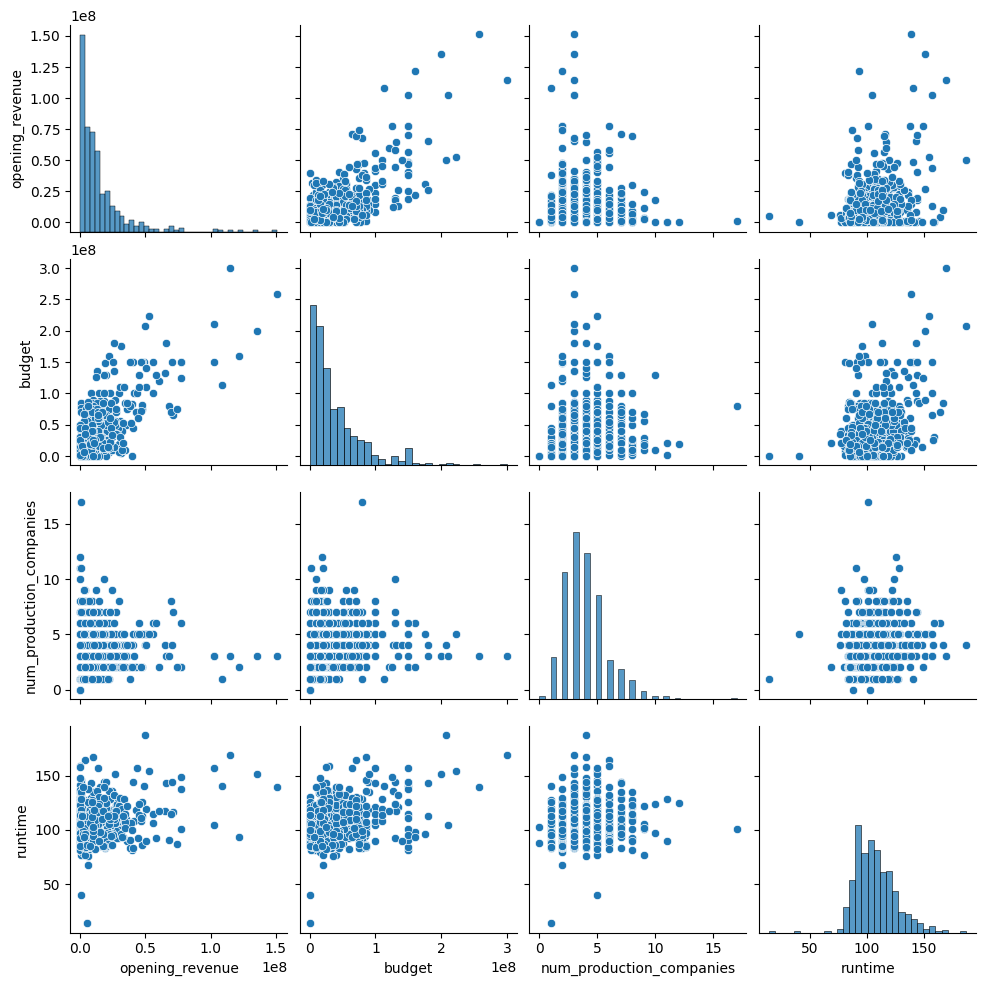
\includegraphics[width=\columnwidth]{pairs_plot}}
		\caption{Pairs plot, initially selected continuous variables.}
	\end{center}
\end{figure}

\begin{figure}[H]
	\begin{center}
		\centerline{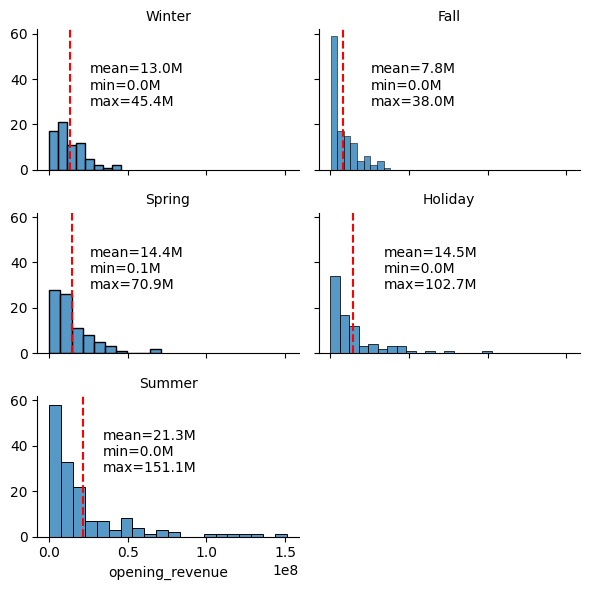
\includegraphics[scale=0.5]{season_revenue}}
		\caption{Distribution of opening revenue by season}
	\end{center}
\end{figure}

\begin{figure}[H]
	\begin{center}
		\centerline{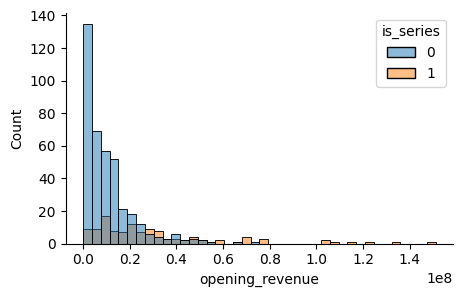
\includegraphics[scale=0.6]{is_series}}
		\caption{Distribution of opening revenue, series vs. non-series}
	\end{center}
\end{figure}

\begin{figure}[H]
	\begin{center}
		\centerline{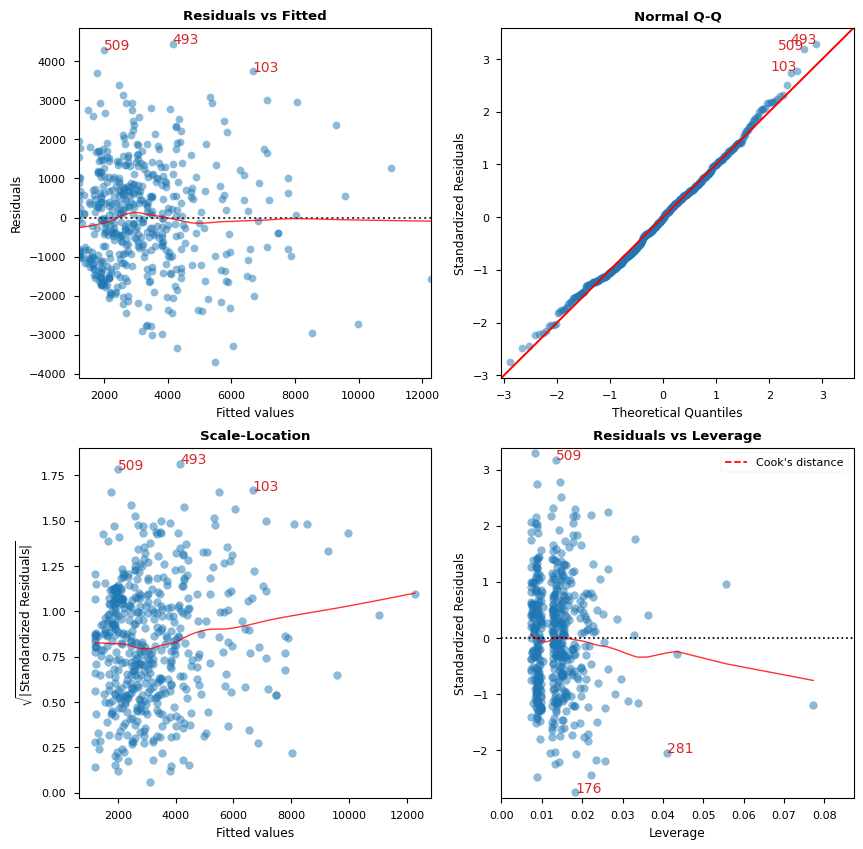
\includegraphics[scale=0.4]{initial_diagnostics}}
		\caption{Residual diagnostics, initial model}
	\end{center}
\end{figure}

\begin{figure}[H]
	\begin{center}
		\centerline{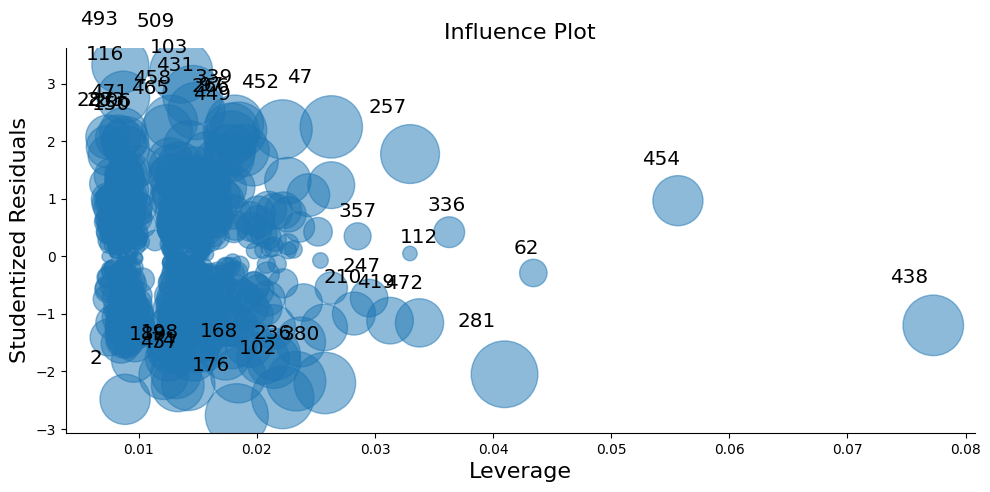
\includegraphics[width=\columnwidth]{influence_plot}}
		\caption{Influence plot (size based on DFFITS)}
	\end{center}
\end{figure}

\begin{figure}[H]
	\begin{center}
		\centerline{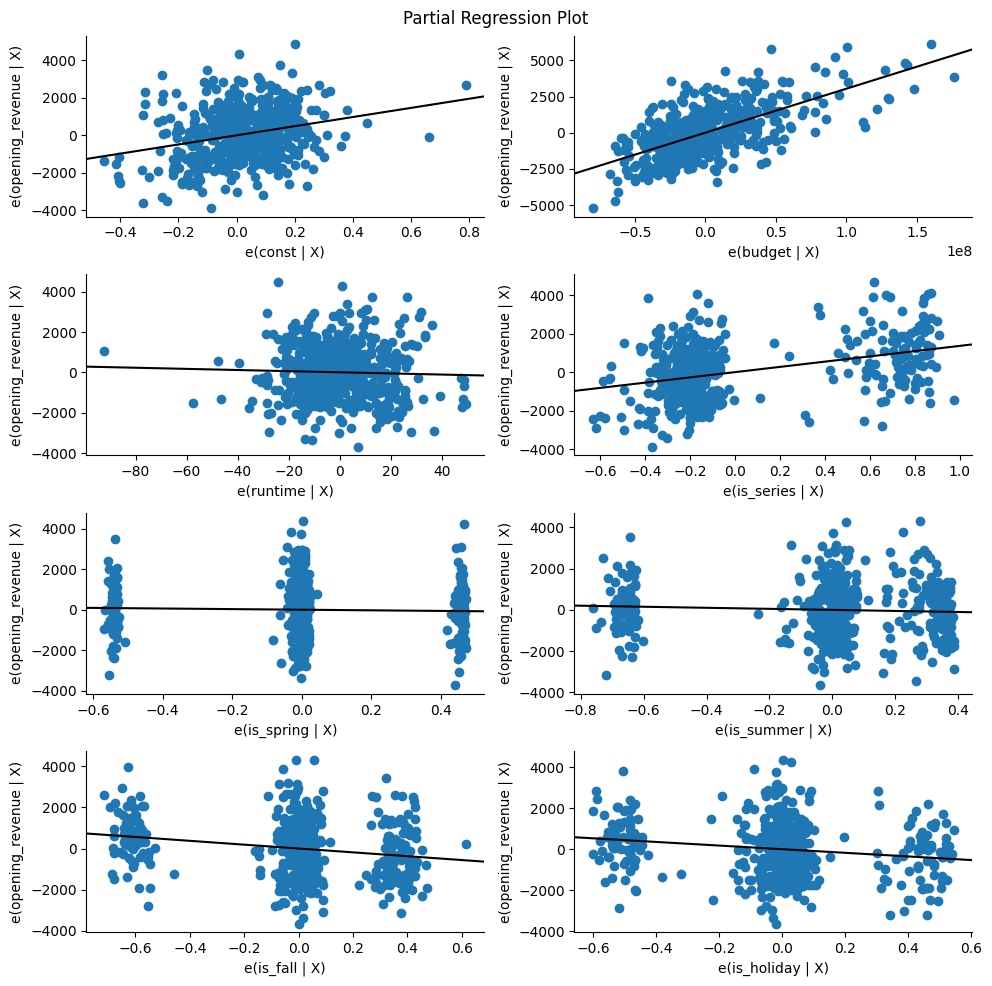
\includegraphics[width=\columnwidth]{partial_regression}}
		\caption{Partial Regression Plots}
	\end{center}
\end{figure}

\section{Analyses}

\begin{table}[H]
\caption{DFFITS results}
\begin{tabular}{llr}
\toprule
obs & release & dffits \\
\midrule
281 & Superman Returns & -0.42 \\
176 & Basic Instinct 2 & -0.38 \\
509 & Wild Hogs & 0.38 \\
102 & Son of the Mask & -0.37 \\
47 & Harry Potter and the Goblet of Fire & 0.37 \\
380 & Evan Almighty & -0.36 \\
438 & Pirates of the Caribbean: At World's End & -0.35 \\
103 & Star Wars: Episode III - Revenge of the Sith & 0.34 \\
236 & Letters from Iwo Jima & -0.34 \\
452 & Shrek the Third & 0.33 \\
257 & Pirates of the Caribbean: Dead Man's Chest & 0.33 \\
339 & 300 & 0.31 \\
431 & Norbit & 0.31 \\
493 & The Simpsons Movie & 0.31 \\
97 & Saw II & 0.30 \\
266 & Saw III & 0.29 \\
168 & An Inconvenient Truth & -0.28 \\
449 & Saw IV & 0.28 \\
5 & Alone in the Dark & -0.27 \\
74 & Memoirs of a Geisha & -0.27 \\
458 & Superbad & 0.27 \\
457 & Sunshine & -0.26 \\
116 & The Exorcism of Emily Rose & 0.26 \\
395 & Happily N'Ever After & -0.26 \\
224 & Ice Age: The Meltdown & 0.25 \\
494 & The Ultimate Gift & -0.25 \\
228 & Jackass Number Two & 0.25 \\
465 & The Bourne Ultimatum & 0.25 \\
198 & Dreamgirls & -0.24 \\
2 & A Sound of Thunder & -0.24 \\
346 & Alvin and the Chipmunks & 0.23 \\
454 & Spider-Man 3 & 0.23 \\
\bottomrule
\end{tabular}
\end{table}

\begin{table}[H]
\caption{DFBETAs, budget (top 10 observations)}
\begin{tabular}[t]{l L{0.5\linewidth} rr}
\toprule
obs & release & budget & dfbeta \\
\midrule
281 & Superman Returns & 223000000 & -0.35 \\
438 & Pirates of the Caribbean: At World's End & 300000000 & -0.32 \\
257 & Pirates of the Caribbean: Dead Man's Chest & 200000000 & 0.26 \\
380 & Evan Almighty & 175000000 & -0.26 \\
452 & Shrek the Third & 160000000 & 0.22 \\
454 & Spider-Man 3 & 258000000 & 0.21 \\
258 & Poseidon & 160000000 & -0.19 \\
47 & Harry Potter and the Goblet of Fire & 150000000 & 0.19 \\
105 & Stealth & 135000000 & -0.17 \\
472 & The Golden Compass & 180000000 & -0.17 \\
\bottomrule
\end{tabular}
\end{table}

\begin{table}[H]
\caption{DFBETAs, is\_series (top 10 observations)}
\begin{tabular}[t]{l L{0.5\linewidth} rr}
\toprule
obs & release & is\_series & dfbeta \\
\midrule
236 & Letters from Iwo Jima & 1 & -0.22 \\
97 & Saw II & 1 & 0.21 \\
266 & Saw III & 1 & 0.21 \\
449 & Saw IV & 1 & 0.20 \\
168 & An Inconvenient Truth & 1 & -0.20 \\
176 & Basic Instinct 2 & 1 & -0.20 \\
228 & Jackass Number Two & 1 & 0.18 \\
103 & Star Wars: Episode III - Revenge of the Sith & 1 & 0.17 \\
339 & 300 & 1 & 0.17 \\
102 & Son of the Mask & 1 & -0.17 \\
\bottomrule
\end{tabular}
\end{table}


\section{Replication Data and Code}
\label{a:code}
The repo \mbox{https://github.com/cons-code/MATH-5500} contains replication data and code.
\end{document}